\documentclass[UTF8,zihao=-4]{ctexbeamer}
\usepackage{multimedia}
\usepackage{hyperref}

\usepackage{listings}

%% 所要粘贴代码的编程语言
%\lstloadlanguages{}

%% 设置listings宏包的一些全局样式
%% 参考http://hi.baidu.com/shawpinlee/blog/item/9ec431cbae28e41cbe09e6e4.html
\lstset{
	showstringspaces=false,              %% 设定是否显示代码之间的空格符号
	numbers=left,                        %% 在左边显示行号
	numberstyle=\tiny,                   %% 设定行号字体的大小
	basicstyle=\footnotesize,                    %% 设定字体大小\tiny, \small, \Large等等
	keywordstyle=\color{blue!70}, commentstyle=\color{red!50!green!50!blue!50},
	%% 关键字高亮
	frame=shadowbox,                     %% 给代码加框
	rulesepcolor=\color{red!20!green!20!blue!20},
	escapechar=`,                        %% 中文逃逸字符,用于中英混排
	xleftmargin=2em,xrightmargin=2em, aboveskip=1em,
	breaklines,                          %% 这条命令可以让LaTeX自动将长的代码行换行排版
	extendedchars=false                  %% 这一条命令可以解决代码跨页时,章节标题,页眉等汉字不显示的问题
}

\usetheme{Madrid}
%\useoutertheme{miniframes}

\usecolortheme{orchid}
\title{程序的基本结构}
\author{高星}
\institute{湖南潇湘技师学院~湖南九嶷职院}
\date{2018.09.14}
\begin{document}
\begin{frame}[plain]
		\maketitle
\end{frame}

\begin{frame}
\begin{columns}
\column[t]{0.3\textwidth}
\column[t]{0.7\textwidth}
\tableofcontents[hideallsubsections]
\end{columns}
\end{frame}

\section{数控编程的坐标系}
\subsection{教学目标}
\begin{frame}{教学目标}
\begin{columns}
	\column{.2\textwidth}
	\column{.8\textwidth}
	\begin{enumerate}
	\item 掌握数控程序的组成与结构。
	\item 掌握数控编程的方法;
	\item 掌握编写数控程序的基本思路;
	\item 了解数控常见指令;
\end{enumerate}
\end{columns}
\end{frame}

\begin{frame}{数控机床的坐标系}
	\begin{columns}
		\column{.4\textwidth}
		\begin{enumerate}
			\item 机床坐标系的定义
			\item 机床坐标系的规定 
			\item 机床坐标系的方向
		\end{enumerate} 
		\column{.6\textwidth}
		\begin{figure}
			\centering
			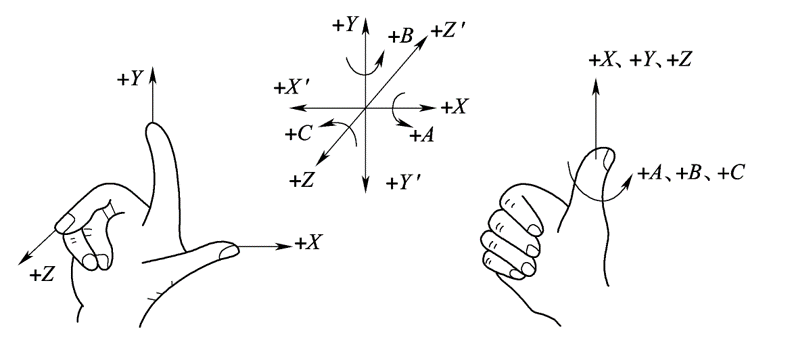
\includegraphics[width= \linewidth]{image/1-22}
			%    	\caption{}
			\label{fig:1-22}
		\end{figure}
	\end{columns}
\end{frame}

\begin{frame}{确定机床坐标系的顺序}
	\begin{columns}
		\column{.3\textwidth}
		\begin{enumerate}
			\item Z轴方向
			\item X轴方向 
			\item Y轴方向
			\item 旋转轴方向
		\end{enumerate} 
		\column{.7\textwidth}
		\begin{figure}
			\centering
			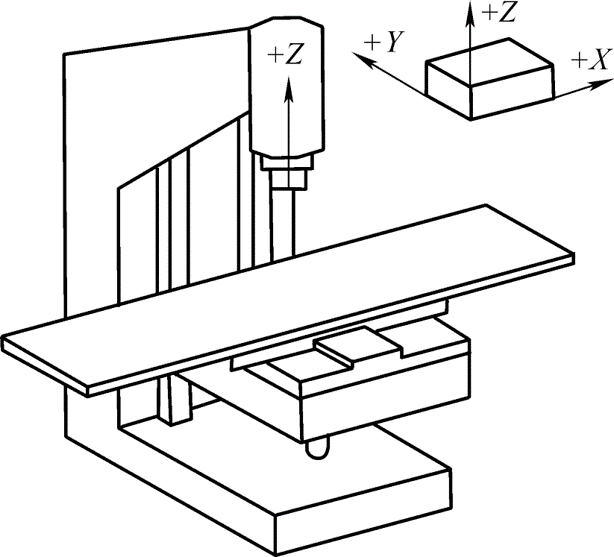
\includegraphics[width= 0.5\linewidth]{image/1-23}
			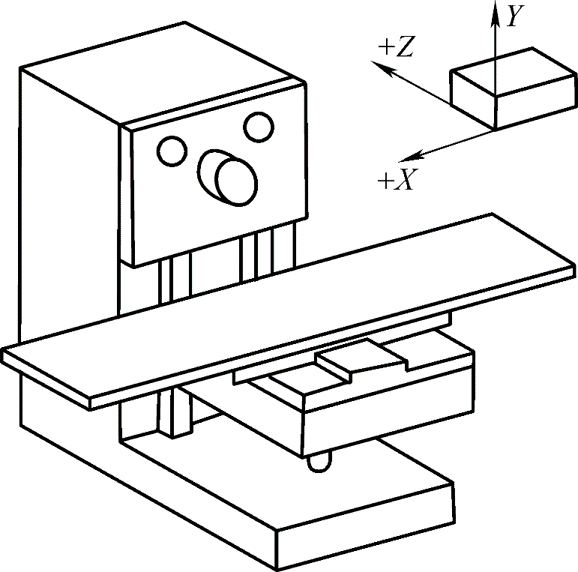
\includegraphics[width= 0.5\linewidth]{image/1-24}
			%    	\caption{}
			\label{fig:1-24}
		\end{figure}
	\end{columns}
\end{frame}

\begin{frame}{机床原点与机床参考点}
 
\begin{block}{ 机床原点}
	机床原点(亦称为机床零点)是机床上设置的一个固定的点,即机床坐标系的原点
\end{block} 

\begin{block}{ 机床参考点}
	机床参考点是数控机床上一个特殊位置的点,通常,第一参考点一般位于靠近机床零点的位置,并由机械挡块来确定其具体的位置。
\end{block} 


机床参考点与机床原点的距离由系统参数设定,其值可以是零,如果其值为零则表示机床参考点和机床零点重合。

\end{frame}

\begin{frame}{工件坐标系}
\begin{block}{ 工件坐标系}
	根据零件图样建立的坐标系称为工件坐标系(亦称编程坐标系)
\end{block}

\begin{block}{ 工件坐标系的原点}
	工件坐标系原点亦称编程坐标系原点,该点是指工件装夹完成后,选择工件上的某一点作为编程或工件加工的原点。
\end{block}	
\end{frame}

\begin{frame}{工件坐标系原点的选择 }
\begin{enumerate}
	\item 工件坐标系原点应选在零件图的基准尺寸上;
	\item 工件坐标系原点应尽量选在精度较高的工件表面上;
	\item Z轴方向上的工件坐标系原点,一般取在工件的上表面;
	\item 当工件对称时,一般以工件的对称中心作为XY平面的原点;
	\item 当工件不对称时,一般取工件其中的一个垂直交角处作为工件原点,
\end{enumerate}
\begin{figure}
	\centering
	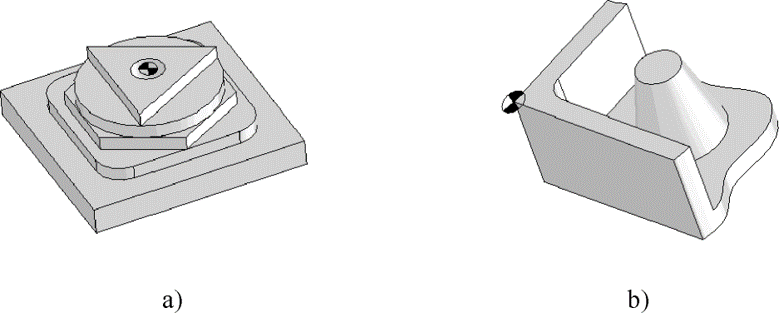
\includegraphics[width= 0.6\linewidth]{image/2-1}
	%    	\caption{}
	\label{fig:1-24}
\end{figure}
\end{frame}

\begin{frame}{其他 }
	\begin{enumerate}
		\item 零点偏置/零点偏移;
		\item 局部坐标系;
		\item 极坐标系;
		\item 工件坐标系的设定。
	\end{enumerate}
\end{frame}


\section{数控程序的结构}

\begin{frame}[fragile]{程序展示}
\begin{lstlisting}
O1;
N10G91G28Z0;
N20T1M6;
N30G54G17G40G49G90;
N40M3S500;
N50G1G43Z100.F2000H1;
N60X-50Y0;
N70Z3;
N80Z-5F200;
N90G2I50;
N100G1G49Z100;
N110M5;
N120M30;
\end{lstlisting}
\end{frame}

\begin{frame} {程序结构}
\begin{enumerate} 
    \item 程序号\\
    程序号写在程序的最前面,必须单独占一行
	\item 程序内容\\程序内容是整个程序的核心,它由许多程序段组成,每个程序段由一个或多个指令构成,它表示数控机床的全部动作。
	\item 程序结束标记 \\程序结束通过M指令来实现,它必须写在程序的最后   。
    \item 程序段的组成\\
    字—地址程序段格式:
    
    \begin{figure}
        \centering
        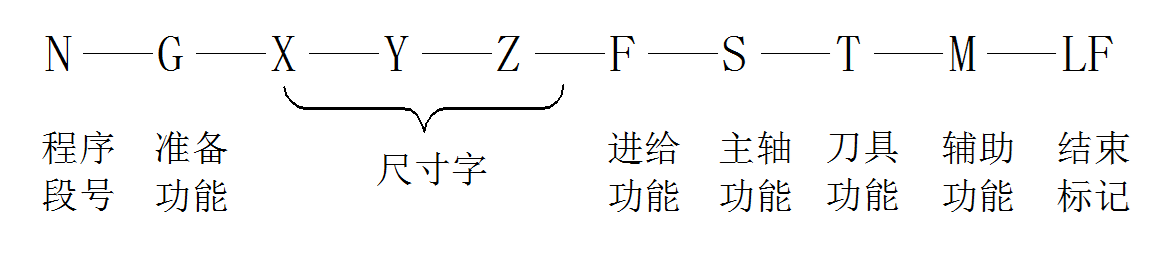
\includegraphics[width= \linewidth]{image/1-25}
    \end{figure}
    
\end{enumerate}
\end{frame}

\begin{frame}[fragile] {程序结构}
         \begin{figure}
       \centering
       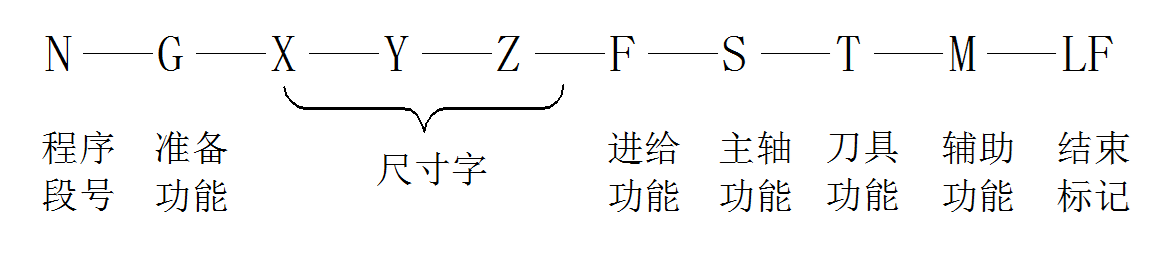
\includegraphics[width= \linewidth]{image/1-25}
   \end{figure}
    \begin{enumerate} 
        \item 序段号  ;
        \item 程序段内容 ;
        \item 程序段结束;
        \item 程序段的斜杠跳跃;
        \item 程序段注释 。     
    \end{enumerate}
\begin{lstlisting}
例  O0001;                    (程序号)
G21 G17 G40 G49 G80 G90;
T01 M06;                       (换刀指令)
……
\end{lstlisting}
\end{frame}


\section{数控程序的指令}

\begin{frame}{数控程序的指令}
 准备功能
 
 准备功能也叫G功能或G指令,是用于数控机床做好某些准备动作的指令。它由地址G和后面的两位数字组成,从G00到G99共有100种G指令 。 
\begin{itemize}
	\item  G0 G1 G2 G3
 \item G17 G18 G19
 \item G54 G55 G56 G57 G58 G59 
 \item  G40 G41 G42
 \item  G90 G91
 \item  G43 G44 G49
 \item  G74 G74 G80-G89
 \item  其他
\end{itemize}
 
\end{frame}

\begin{frame}{数控程序的指令}
	辅助功能
	
    辅助功能也叫M功能或M指令。它由地址M和后面的两位数字组成,从M00-M99共100种 。
    \begin{itemize}
		\item  M0 M1 M2 M30
		\item M3 M4 M5
		\item M6
		\item M7 M8 M9
		\item  M98 M99
		\item  其他
	\end{itemize}
	
\end{frame}

\begin{frame}{数控程序的指令}
	其他指令
	
	\begin{itemize}
        \item X~Y~Z~A~B~C~U~V~W(坐标功能)
		\item  T(刀具功能)
		\item S(主轴功能)
		\item F(进给功能)
		\item  其他
	\end{itemize}
	
\end{frame}

\begin{frame}{数控程序的指令}
	
	
	\begin{itemize}
		\item 指令分组\\所谓指令分组,就是将系统中不能同时执行的指令分为一组,并以编程号区别。
        
         \item 模态指令/非模态指令\\模态指令(又称为续效指令)表示该指令在一个程序段中一经指定,在接下来的程序段中一直持续有效,直到出现同组的另一个指令时,该指令才失效。
         
		\item 开机默认指令\\
        常见的开机默认指令有G01、G17、G40、G49、G54、G80、G90、G94、G97等。如当程序中没有G96或G97指令,用指令“M03 S200;”指定的正转转速是200r/min。 
	\end{itemize}
\end{frame}


\section{数控编程的方式}
\begin{frame}{数控编程的方式}
\begin{enumerate}
    \item 手工编程
    
    利用一般的计算工具,通过各种数学方法,人工进行刀具轨迹的运算,并进行指令编制。该方式比较简单,容易掌握。适用于中等复杂程度、计算量不大的零件编程,对机床操作人员来讲必须掌握的。
    
    手工编程在目前仍是广泛采用的编程方式,即使在自动编程高速发展的将来,手工编程的重要地位也不可取代。
    
    \item 自动编程  
    
    利用计算机(含外围设备)和相应的前置、后置处理程序对程序对零件源程序进行处理,以得到加工程序单各数控带的一种编程方式。
    
    对于曲线轮廓、三维曲面等复杂型面。一般采用自动编程。
    
    在工作站或个人PC上利用CAD/CAM系统进行零件的设计、分析及加工编程。它适用于各类柔性制造系统(FMS)和计算机集成制造系统(CIMS)。
    
\end{enumerate}
\end{frame}

\section{编写程序的基本思路}
\begin{frame}{编写程序的基本思路}
程序初始化(安全保护)--------辅助准备(换刀,主轴启动,切削液开)--------定位到起刀点--------快速下刀--------工进下刀--------走加工轮廓--------提刀---------快速提刀到安全平面-------程序结束(换刀,主轴停止,切削液关,程序返回等)
\end{frame}


\section*{课堂小结}
\begin{frame}{课堂小结}
\begin{enumerate}
    \item 数控编程的坐标系及假设;
    \item 数控程序的结构;
    \item 数控程序的指令;
    \item 数控编程的方式;
    \item 编写程序的基本思路。
\end{enumerate}
\end{frame}

\begin{frame}{作业}
\begin{enumerate}
    \item 写出数控程序的基本结构。
    \item 数控编程的方式有哪些?
\end{enumerate}
\end{frame}

\begin{frame}[plain]
\vfill

\centering \huge 谢谢大家!

\vfill

\flushleft \footnotesize   
~~~QQ:32731964\\
~~~TEL:18974681118\\
%~~~课件下载:\\
%~~~https://github.com/gnixoag/myworks2017/tree/master/jiaoshichengzhang

\end{frame}

\end{document} 
